This component acts as a registry for out-going commands and reports (namely for commands or report which have been loaded into an OutManager).

The OutRegistry is defined as an extension of the Base Component of section \ref{sec:BaseCmp}. It has two functions: (a) it keeps track of an out-going command's or report's state; and (b) it stores the out-going command's or report's enable state.

The OutRegistry maintains a list of the last N commands or reports to have been loaded in all OutManagers in an application. The OutRegistry maintains the state of each such command or report. The command's or report's state in the OutRegistry can have one of the following values:
\begin{itemize}
\item PENDING: the command or report is waiting to be sent
\item ABORTED: the command or report was aborted because it was disabled when it was loaded
\item TERMINATED: the command or report has been passed to the OutStream
\end{itemize}
The value of N (the maximum number of items which can be tracked by the OutRegistry) is fixed and is an initialization parameter.

An OutComponent is first registered with the OutRegistry when it is loaded into the OutManager through the latter \texttt{Load} operation. Subsequently, the information in the OutRegistry is updated by the OutManagers every time a command or report is executed. Normally, a command's or report's state in the OutRegistry eventually becomes either ABORTED or TERMINATED. The only situation where this is not the case is\footnote{This exception could be avoided if the OutRegistry were notified of the reset of the OutManager. This is not done for reasons of simplicity and because it is expected that applications which reset an OutManager will normally also reset the OutRegistry.}: if an OutManager is reset, then the state of a command or report that was in state PENDING at the time the OutManager was reset will remain equal to PENDING.

The OutRegistry uses the identifier attribute (see sections \ref{sec:CmdAttributes} and \ref{sec:RepAttributes}) as the key through which the command or report state is stored.

\begin{figure}[h]
 \centering
 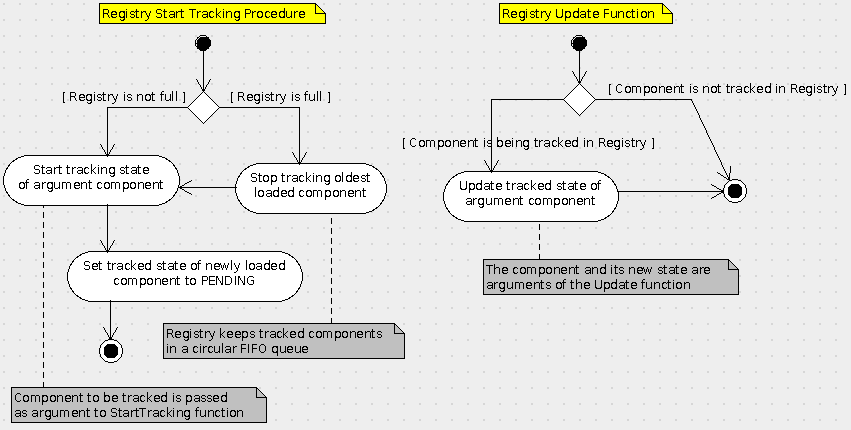
\includegraphics[scale=0.5,keepaspectratio=true]{RegistryStartTrackingAndUpdate.png}
 \caption{The Registry Start Tracking and Registry Update Procedures}
 \label{fig:RegistryStartTrackingAndUpdate}
\end{figure}

In order to perform the tasks described above, the OutRegistry offers two operations: \texttt{StartTracking} and \texttt{Update}. These operations run the procedures Registry Start Tracking and Registry Update shown in figure \ref{fig:RegistryStartTrackingAndUpdate}. Operation \texttt{StartTracking} is performed by the \texttt{Load} operation of an OutManager to register an OutComponent with the OutRegistry. Operation \texttt{Update} is performed by the \textit{Execution Procedure} of an OutManager to ask the OutRegistry to update its information about an OutComponent's state.

The OutRegistry stores the enable state of out-going commands and reports. The enable state of out-going command and reports can be controlled at three levels: 
\begin{itemize}
\item[(a)] At the level of the service type (all commands or reports of a certain type are disabled)
\item[(b)] At the level of the service sub-type (all commands or reports matching a certain [type, sub-type] pair are disabled)
\item[(c)] At the level of the discriminant (all commands or reports matching a certain [type, sub-type, discriminant] triplet are enabled or disabled)
\end{itemize}
The enable state of a particular command or report is derived from these three enable levels by running the \textit{Enable State Determination Procedure} of figure \ref{fig:EnableStateDetermination}.

The OutRegistry offers an API through which all three levels of enable state can be set and read. By default, all enable states are set to: “enabled”. The enable states are configuration parameters for the OutRegistry which are reset to: “enabled” every time the component is reset.

As discussed in section \ref{sec:OutComponent}, by default, the Enable Check of an out-going command or report determines whether the command or report is enabled or not by reading its enable status from the OutRegistry. 

\begin{figure}[H]
 \centering
 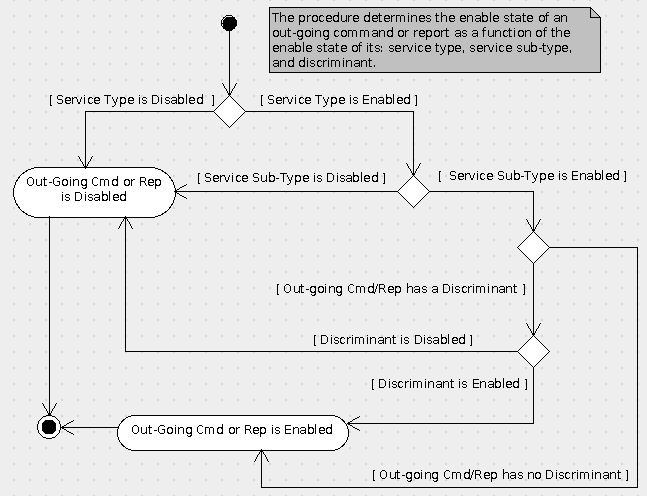
\includegraphics[scale=0.5,keepaspectratio=true]{EnableStateDetermination.png}
 \caption{The Enable State Determination Procedure}
 \label{fig:EnableStateDetermination}
\end{figure}

